% !TEX encoding = UTF-8
% !TEX TS-program = pdflatex
% !TEX root = ../tesi.tex

%**************************************************************
\chapter{Codifica}
\label{cap:codifica}
%**************************************************************

La codifica del prodotto, come descritto nel capitolo 2 è stata suddivisa in sprint di sviluppo che corrispondono a circa 4-5 giorni lavorativi dove vengono implementati parte delle user stories indicate nel product backlog. Per ogni sprint verrano descritti lo Sprint Backlog e le Soluzioni che sono state implementate e i seguenti eventi: \textbf{Sprint Review} e \textbf{Backlog refinement}.
Infine verranno elencati i possibili ritardi, i problemi riscontrati e le soluzioni trovate. Ogni sprint è stato identificato da un codice univoco e da un titolo. In questo progetto gli sprint individuati sono i seguenti:
\begin{itemize}
	\item \textbf{S1: Struttura dello stato e dell'architettura Redux};
	\item \textbf{S2: Componenti grafici e container Redux};
	\item \textbf{S3: Parser JSON e adapter};
	\item \textbf{S4: Caricamento parziale}.
\end{itemize}

\section{S1: Struttura dello stato e dell'architettura Redux}
\textbf{Durata:} \textit{5 giorni} \\
Nel primo sprint di sviluppo sono stati implementati i requisiti considerati più importanti per porre delle solide basi dell'applicazione; in particolare la progettazione e codifica della struttura dello stato e l'architettura di Redux.

\subsection{Sprint Backlog}
In particolare sono stati implementati questi requisiti.
\begin{longtable} {
		|>{}p{10mm}| 
		|>{}p{90mm}|
		|>{}p{15mm}|
		|>{}p{15mm}|
		|>{}p{15mm}|
		>{}p{0mm}}
	\hline
	\textbf{Id} & \textbf{Descrizione} & \textbf{Tipo} \\ \hline
	R1.0 & Definizione dello stato dell'applicazione & O \\ \hline
	R1.0.1 & Sviluppo TableState        & O\\ \hline
	R1.0.2 & Sviluppo NodeDimensions    & O\\ \hline
	R1.0.3 & Sviluppo BodyCells         & O\\ \hline
	R1.0.4 & Sviluppo HeaderAction      & O\\ \hline
	R1.0.5 & Sviluppo NodeActionType    & O\\ \hline
	R1.1   & Definizione architettura Redux & O\\ \hline
	R1.1.1 & Sviluppo TableStateSlice    & O\\ \hline
	R1.1.2 & Sviluppo di Thunk & O\\ \hline
	R1.1.3 & Sviluppo delle Actions & O\\ \hline
	R1.1.4 & Sviluppo dei Reducers & O\\ \hline
\end{longtable}

\subsection{Soluzioni implementate}
Ho realizzato i seguenti \verb|package|:
\begin{itemize}
	\item \verb|redux|
	\item \verb|redux.slices|
	\item \verb|redux.thunks|
	\item \verb|redux.state|
	\item \verb|entities|
\end{itemize}

\subsubsection{redux.slice}
\begin{lstlisting}[caption={TableState}, label={lst:tablestate}, language=Kotlin]
object TableStateSlice {
	data class State(
	  val cols: ArrayList<ArrayList<DimensionsNode>> = ArrayList(),
	  val rows: ArrayList<ArrayList<DimensionsNode>> = ArrayList(),
	  val cells: ArrayList<ArrayList<BodyCells>> = ArrayList(),
	  val rowActions: ArrayList<ArrayList<HeaderAction>> = ArrayList(),
	  val colActions: ArrayList<ArrayList<HeaderAction>> = ArrayList(),
	  val isLoading: Boolean = false,
	)
	
	private val initTableState = InitState()
	fun initTable() : RThunk = initTableState
	
	class UpdateCells(val cells: ArrayList<ArrayList<BodyCells>>): RAction
	class UpdateRows(val rows: ArrayList<ArrayList<DimensionsNode>>): RAction
	class UpdateCols(val cols: ArrayList<ArrayList<DimensionsNode>>): RAction
	class SetIsLoading(val b: Boolean): RAction
	class UpdateRowActions(val n: ArrayList<ArrayList<HeaderAction>>): RAction
	class UpdateColActions(val n: ArrayList<ArrayList<HeaderAction>>): RAction
	
	fun reducer(state: State = State(), action: RAction) : State {
		return when (action) {
			is UpdateCells -> state.copy(cells = action.cells)
			is UpdateRows -> state.copy(rows = action.rows)
			is UpdateCols -> state.copy(cols = action.cols)
			is SetIsLoading -> state.copy(isLoading = action.b)
			is UpdateRowActions -> state.copy(rowActions = action.n)
			is UpdateColActions -> state.copy(colActions = action.n)
			else -> state
		}
	}
}
\end{lstlisting}

\subsubsection{redux.thunks}
La classe \verb|InitState| si occuperà di riempire lo stato della tabella con il risultato della richiesta HTTP non ancora implementata.
\begin{lstlisting}[caption={TableState}, label={lst:tablestate}, language=Kotlin]
class InitState : RThunk {
	override fun invoke(dispatch: (RAction) -> WrapperAction, getState: () -> AppState): WrapperAction {
		val mainScope = MainScope()
		mainScope.launch {
			// val res : TableState = fetchCreavistaJson()
			dispatch(TableStateSlice.UpdateRows(res.rows))
			dispatch(TableStateSlice.UpdateCols(res.cols))
			dispatch(TableStateSlice.UpdateCells(res.cells))
			dispatch(TableStateSlice.UpdateRowActions(res.rowAction))
			dispatch(TableStateSlice.UpdateColActions(res.colAction))
		}
		return nullAction
	}
}
\end{lstlisting}

\subsubsection{redux.state}
Lo stato dell'applicazione è definito in modo che sia completamente modulare. Infatti la \verb|data class AppState| contiene un'istanza dello stato di \verb|TableStateSlice|. In questo modo in un futuro, se si vorrà espandere questo componente si potrà semplicemente aggiungere un nuovo "slice" e modificare questo file in modo da collegarlo a \verb|AppState|.
\begin{lstlisting}[caption={TableState}, label={lst:tablestate}, language=Kotlin]
data class AppState (
  val tableState: TableStateSlice.State = TableStateSlice.State()
)

// funzioni per collegare AppState a TableStateSlice
fun rootReducer(): Reducer<AppState, RAction> = getRootReducers(
  mapOf(
    AppState::tableState to TableStateSlice::reducer
  )
)

fun <S, A, R> getRootReducers(reducers: Map<KProperty1<S, R>, Reducer<*, A>>): Reducer<S, A> {
	return combineReducers(reducers.mapKeys { it.key.name })
}
\end{lstlisting}

\subsubsection{entities}
\paragraph*{TableState} \mbox{} \\
L'entità \verb|TableState| è la \verb|data class| che contiene l'intero stato dell'applicazione. Al suo interno sono presenti tutte le informazioni necessarie per la corretta renderizzazione della tabella pivot.
\begin{lstlisting}[caption={TableState}, label={lst:tablestate}, language=Kotlin]
data class TableState(
  val cols: ArrayList<ArrayList<DimensionsNode>>,
  val rows: ArrayList<ArrayList<DimensionsNode>>,
  val cells: ArrayList<ArrayList<BodyCells>>,
  val rowAction: ArrayList<ArrayList<HeaderAction>>,
  val colAction: ArrayList<ArrayList<HeaderAction>>
)
\end{lstlisting}

\paragraph*{DimensionsNode} \mbox{} \\
L'entità \verb|DimensionsNode| è la \verb|data class| che contiene le informazioni riguardanti una cella d'intestazione della tabella pivot.
\begin{lstlisting}[caption={DimensionsNode}, label={lst:dimensionsnode}, language=Kotlin]
data class DimensionsNode(
  var id: String,
  var label: String,
  var level: Int? = null,
  var childDepth: Int? = null,
  var path: List<String>? = null,
  var actionType: NodeActionType = NodeActionType.NULL,
  var isChild: Boolean = false
)
\end{lstlisting}

\paragraph*{HeaderAction} \mbox{} \\
L'entità \verb|HeaderAction| è la \verb|data class| che contiene le informazioni riguardanti i pulsanti che si occupano di aprire intere colonne o righe di dimensioni nella TableActionUI.
\begin{lstlisting}[caption={HeaderAction}, label={lst:headeraction}, language=Kotlin]
data class HeaderAction(
  val actionType: NodeActionType,
  val dim: Int,
  val depth: Int,
)
\end{lstlisting}

\paragraph*{NodeActionType} \mbox{} \\
L'entità \verb|HeaderAction| è una \verb|enum class| che definisce il tipo di azione che può essere eseguita da una cella.
\begin{lstlisting}[caption={NodeActionType}, label={lst:nodeactiontype}, language=Kotlin]
enum class NodeActionType(val type: String) {
  EXPAND("E"),
  COLLAPSE("C"),
  NULL("")
}
\end{lstlisting}

\paragraph*{BodyCells} \mbox{} \\
L'entità \verb|BodyCells| è la \verb|data class| che contiene le informazioni riguardanti le celle che contengono i dati della tabella.
\begin{lstlisting}[caption={BodyCells}, label={lst:bodycells}, language=Kotlin]
data class BodyCells(
  val value: Int,
  val cPath: List<String>,
  val rPath: List<String>
)
\end{lstlisting}

\subsection{Sprint Review}
Niente da segnalare.

\subsection{Backlog refinement}
Il Product Backlog non è stato modificato.

\subsection{Problemi riscontrati}
Implementare correttamente l'architettura Redux è risultato difficoltoso a causa della mia inesperienza con la libreria e la mancanza di documentazione relativa a \verb|kotlin-redux|. Questi problemi non hanno però causato rallentamenti nell'implementazione degli altri requisiti dello Sprint Backlog.

\newpage

\section{S2: Componenti grafici e container Redux}
\textbf{Durata:} \textit{5 giorni} \\
Nel secondo sprint di sviluppo ho lavorato sull'interfaccia grafica e quindi i componenti React e i relativi container Redux.

\subsection{Sprint Backlog}
\begin{longtable} {
		|>{}p{10mm}| 
		|>{}p{90mm}|
		|>{}p{15mm}|
		|>{}p{15mm}|
		|>{}p{15mm}|
		>{}p{0mm}}
	\hline
R2.0   & \textbf{Definizione dei componenti} & O\\ \hline
R2.1   & Sviluppo dei componenti React 		  & O\\ \hline
R2.1.1 & Sviluppo di TableView                & O\\ \hline
R2.1.2 & Sviluppo di TableHeaderView          & O\\ \hline
R2.1.3 & Sviluppo di TableSidebarView         & O \\ \hline
R2.1.4 & Sviluppo di TableBodyView            & O\\ \hline
R2.1.5 & Sviluppo di TableActionUI            & O\\ \hline
R2.1.6 & Sviluppo di TableLabelView            & O\\ \hline
R2.2   & Sviluppo dei container Redux         & O  \\ \hline
R2.2.2 & Sviluppo di TableController          & O   \\ \hline
R2.2.3 & Sviluppo di TableHeaderController    & O      \\ \hline
R2.2.4 & Sviluppo di TableSidebarController   & O      \\ \hline
R2.2.5 & Sviluppo di TableBodyController      & O   \\ \hline
R2.2.6 & Sviluppo di TableLabelController   & O      \\ \hline
R2.2.7 & Sviluppo di TableActionUIController      & O   \\ \hline
\end{longtable}

\subsection{Soluzioni implementate}
Le componenti grafiche realizzate sono le seguenti: \\
\begin{minipage}{\linewidth}
	\makebox[\linewidth] {
		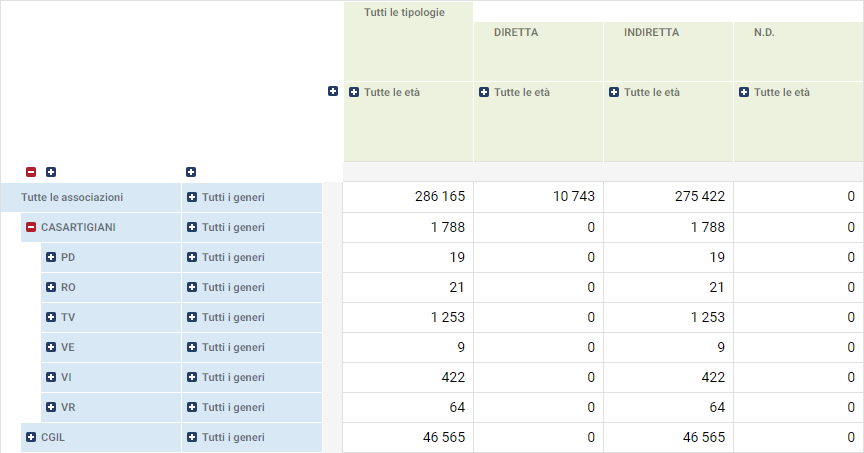
\includegraphics[scale=0.60]{./immagini/table-pivot.png}
	}
\end{minipage}
\\
\\
Per rendere l'interfaccia utente chiara e utilizzabile da un dispositivo mobile ho realizzato le dimensione dimensioni della tabella in modo che possano essere nascoste. Inoltre ogni cella di intestazione può essere cliccata per attivare l'azione, questo perchè cliccare un pulsante molto piccolo da un dispositivo mobile è risultato difficile nei test manuali effettuati.

\subsubsection{redux.container}
Per ogni componente che richiedeva un collegamento con lo stato di Redux ho realizzato un wrapper che permette di mappare lo stato di Redux alle \emph{props} di un componente React. I wrapper sono stati definiti nel seguente modo:
\begin{lstlisting}[caption={BodyCells}, label={lst:bodycells}, language=Kotlin]
// campi dato dello stato da mappare alle props
private interface StateProps : RProps {
	var rows: ArrayList<DimensionsNode>
	...
}

// funzioni per modificare lo stato da mappare alle props
private interface DispatchProps: RProps {
	var updateRows: (rows: ArrayList<DimensionsNode>) -> Unit
	...
}

val reactComponent: RClass<RComponentProps> =
rConnect<AppState, RAction, WrapperAction, RProps, StateProps, DispatchProps, RComponentProps>(
mapStateToProps = { state, _ ->
	rows = state.tableState.rows
},
mapDispatchToProps = { dispatch, _ ->
	updateRows = { rows -> dispatch(TableStateSlice.UpdateRows(rows)) }
}
)(TableActionUI::class.js.unsafeCast<RClass<RComponentProps>>())
\end{lstlisting}
\subsection{Sprint Review}
Niente da segnalare.

\subsection{Backlog refinement}
Il Product Backlog non è stato modificato.

\subsection{Problemi riscontrati}
All'inizio dello sprint ho realizzato i componenti grafici con una scrittura funzionale, tuttavia dopo aver implementato i container Redux ho notato la presenza di alcuni limitazioni nell'uso di Redux e componenti funzionale di React. Quindi ho riscritto i componenti con una scrittura a classi. Questo problema non ha però causato ritardi gravi. 

\newpage

\section{S3: Parser JSON e adapter}
\textbf{Durata:} \textit{8 giorni} \\
Nel terzo sprint ho realizzato le funzioni per eseguire richieste HTTP e le ho implementate in modo da funzionare correttamente con le funzioni eseguite nel primo sprint. In seguito ho realizzato le \verb|data class @Serializable| per eseguire il parsing del json. Infine ho scritto le funzioni che mi hanno permesso di tradurre i dati ricevuti dall'api nelle strutture dati definite nel primo sprint.
 
\subsection{Sprint Backlog}
\begin{longtable} {
		|>{}p{10mm}| 
		|>{}p{90mm}|
		|>{}p{15mm}|
		|>{}p{15mm}|
		|>{}p{15mm}|
		>{}p{0mm}}
	\hline
	R3.0   & \textbf{Sviluppo parser per JSON dell'API}         & O\\ \hline
	R3.1   & Sviluppo data class @Serializable 	   & O\\ \hline
	R3.1.1 & Sviluppo Gruppo4JSON & O\\ \hline
	R3.1.2 & Sviluppo Gruppo4Data & O\\ \hline
	R3.1.3 & Sviluppo Gruppo4Filter & O\\ \hline
	R3.1.4 & Sviluppo Gruppo4Actions & O\\ \hline
	R3.1.5 & Sviluppo Gruppo4Node & O\\ \hline
	R3.2   & \textbf{Sviluppo adapter da JSON a TableState} & O\\ \hline
	R3.2.1   & Sviluppo funzione convertListOfGruppo4Node() & O\\ \hline
	R3.2.2   & Sviluppo funzione convertTree() & O \\ \hline
	R3.2.3   & Sviluppo funzione convertListOfGruppo4Actions() & O\\ \hline
	R3.2.4   & Sviluppo funzione convertCells() & O\\ \hline
	
	R4.0 & \textbf{Sviluppo funzioni per effettuare richieste HTTP}  & O    \\ \hline
	R4.1   & Sviluppo funzione fetch() & O     \\ \hline
	R4.2   & Sviluppo funzione sendAction() & O    \\ \hline
\end{longtable}

\subsection{Soluzioni implementate}
\subsubsection{Gestione delle richieste all'API}
Il primo passo per utilizzare dei dati reali all'interno della tabella pivot è stato quello di realizzare una funzione per effettuare richieste HTTP alla API di Gruppo4. Per farlo ho utilizzato l'implementazione in Kotlin di \verb|window.fetch|. La funzione risultante è la seguente:
\begin{lstlisting}[caption={Funzione fetch()}, label={lst:bodycells}, language=Kotlin]
suspend fun fetch() {
  val res = window.fetch(url, RequestInit(
    method = "GET",
    credentials = RequestCredentials.Companion.INCLUDE,
    headers = {
      json("Accept" to "application/json")
      json("Content-Type" to "application/json")
    }))
    .await()
    .json()
    .await()

   // Codice identificativo dell'istanza della tabella pivot necessario
   // per le chiamate successive
   INSTANCE_KEY = (res as kotlin.js.Json)["InstanceKey"] as String?
}
\end{lstlisting}

\noindent
La seguente funzione effettua una richiesta HTTP GET alla API di Gruppo4 la quale ritorna il JSON risultante e una chiave necessaria per effettuare le chiamate successive per la corretta tabella pivot. Per le richieste in seguito ad un'azione da parte di un utente ho utilizzato la seguente funzione \verb|sendAction()| che in modo similare alla precedente esegue una richiesta HTTP POST all'API della tabella di un JSON che contiene le seguenti informazioni:
\begin{itemize}
	\item \verb|axis|: può essere "R" o "C" (righe o colonne);
	\item \verb|path|: array identificativo della cella su cui è stata effettuata l'azione.
\end{itemize}
L'implementazione di \verb|sendAction()| è la seguente: 
\begin{lstlisting}[caption={Funzione sendAction()}, label={lst:bodycells}, language=Kotlin]
suspend fun sendAction(body: String, type: String) {
    val res: Any? = window.fetch("$url$INSTANCE_KEY/$type", RequestInit(
      method = "POST",
      body = body,
      credentials = RequestCredentials.Companion.INCLUDE,
      headers = {
        json("Accept" to "application/json")
        json("Content-Type" to "application/json")
      }))
     .await()
     .json()
     .await()
}
\end{lstlisting}

\subsubsection{Entità @Serializable}
Per non dilungare troppo questa sezione mostrerò solo una entità:
\begin{lstlisting}[caption={data class Gruppo4Action}, label={lst:bodycells}, language=Kotlin]
@Serializable
data class Gruppo4Action(
  @SerialName("Action")
  val action: String? = null,
  @SerialName("Dim")
  val dim: Int? = null,
  @SerialName("Depth")
  val depth: Int? = null,
  @SerialName("Path")
  val path: Array<String>? = null
)
\end{lstlisting}
\subsubsection{Funzioni adapter}
Di seguito indico le funzioni principali per eseguire la conversione tra le entità \verb|@Serializable| e le entità dello stato. Dalle seguenti funzioni si può vedere l'utilizzo delle \emph{higher order functions} per semplificare il più possibile il codice.

\begin{lstlisting}[caption={Funzione convertListOfGruppo4Node()}, label={lst:bodycells}, language=Kotlin]
fun convertListOfGruppo4Node(list: ArrayList<Gruppo4Node>?): ArrayList<DimensionsNode>? {
	return list?.map { it.toDimensionsNode() }?.toCollection(ArrayList())
}
\end{lstlisting}

\begin{lstlisting}[caption={Funzione convertListOfGruppo4Actions()}, label={lst:bodycells}, language=Kotlin]
fun convertListOfGruppo4Actions(list: ArrayList<Gruppo4Action>, limit: Int): ArrayList<ArrayList<HeaderAction>> {
	val res: ArrayList<ArrayList<HeaderAction>> = ArrayList()
	var index = 0
	while (index < limit) {
		res.add(index, ArrayList())
		index++
	}
	
	list.groupBy { it.dim }.entries.map {
		val tmpList = it.value.map { c -> c.toHeaderAction() }.toCollection(ArrayList())
		val limit = tmpList.last().depth
		res.set(it.key!!, normaliseListAction(tmpList, limit))
	}
	
	return res
}
\end{lstlisting}

\begin{lstlisting}[caption={Funzione convertCells()}, label={lst:bodycells}, language=Kotlin]
fun convertCells(list: Array<Array<Double>>, rowsPaths: Array<Array<String>>? , colsPaths: Array<Array<String>>?): ArrayList<ArrayList<BodyCells>>? {
	val tmp: ArrayList<ArrayList<BodyCells>> = ArrayList()
	var cellTmp: ArrayList<BodyCells> = ArrayList()
	if (rowsPaths == null || colsPaths == null) {
		return null
	}
	for ((indx, items) in list.withIndex()) {
		val rPath = rowsPaths[indx]
		for ((index, item) in items.withIndex()) {
			cellTmp.add(
			BodyCells(
			value = item.toInt(),
			cPath = colsPaths[index],
			rPath = rPath
			)
			)
		}
		tmp.add(cellTmp)
		cellTmp = ArrayList()
	}
	return tmp
}
\end{lstlisting}

\begin{lstlisting}[caption={Funzione convertTree()}, label={lst:bodycells}, language=Kotlin]
fun convertTree(node: DimensionsNode?, level: Int, currentPath: List<String>, depth: Int): List<DimensionsNode?> =
if (node == null) {
	listOf()
} else {
	val subDimNode = node.subDim
	val action = createActionFor(node.children)
	val newNode = node.setLevel(level).setPath(currentPath).setActionType(action).setDepth(depth)
	(
	listOf(newNode) +
	(
	subDimNode?.flatMap {
		getRow(
		it.setLevel(level + 1),
		level + 1,
		currentPath + it.id,
		if (!node.isChild) depth else 0
		)
	} ?: listOf()
	) +
	(
	node.children?.flatMap {
		getRow(
		it.setLevel(level).setIsChild(true),
		level,
		currentPath.dropLast(1) + it.id,
		depth + 1
		)
	} ?: listOf()
	)
	).sortedWith(compareBy { it?.level })
}
\end{lstlisting}

\begin{lstlisting}[caption={Funzione parseJSON()}, label={lst:bodycells}, language=Kotlin]
fun parseJSON(res: String): TableState {
  val obj = Json.decodeFromString<Gruppo4Json>(res)

  val tableData: ArrayList<ArrayList<BodyCells>> = convertCells(obj.cells, obj.rows?.paths, obj.cols?.paths)!!
  val rowTree = convertListOfGruppo4Node(obj.rows?.tree)
  val colTree = convertListOfGruppo4Node(obj.cols?.tree)

  val rowCells = getCellsFromTree(rowTree !!)
  val colCells = getCellsFromTree(colTree !!)

  val rowNormalisedCells = normaliseList(rowCells)
  val colNormalisedCells = normaliseList(colCells)

  val rowAction = gruppo4actionsToActionType(obj.rows?.actions !!, rowCells.groupBy { it?.level }.size)
  val colAction = gruppo4actionsToActionType(obj.cols?.actions !!, colCells.groupBy { it?.level }.size)

  val rows = rowCells.toCollection(ArrayList())
  val cols = colCells.toCollection(ArrayList())

  return TableState(
    cells = tableData,
    cols = colNormalisedCells,
    rows = rowNormalisedCells,
    colTree = cols,
    rowTree = rows,
    rowAction = rowAction,
    colAction = colAction
  )
}
\end{lstlisting}

\subsection{Sprint Review}
Niente da segnalare.

\subsection{Backlog refinement}
Il Product Backlog non è stato modificato.

\subsection{Problemi riscontrati}
La realizzazione dell'adapter è stata rallentata da cambiamenti della struttura dell'API da parte dell'azienda, infatti la struttura ad albero delle dimensioni della tabella è stata modificata, ogni nodo infatti presenta due tipologie di figli: i nodi graficamente sotto di esso e i nodi graficamente laterali ad esso. I rallentamenti hanno causato una lunghezza dello sprint elevata. La realizzazione dell'adapter ha infatti anche occupato parte della settimana riservata al quarto sprint. I rallentamenti sono dovuti anche alla codifica della funzione \verb|convertTree()| data la sua complessità.

\newpage

\section{S4: Caricamento parziale}
\textbf{Durata:} \textit{4 giorni} \\
Nell'ultimo sprint finale sono state realizzate le funzioni che riguardano il caricamento parziale dei dati della tabella. Tuttavia per alcuni problemi riguardanti l'API fornita da Gruppo4 è stato impossibile realizzare in modo completo la funzionalità del caricamento parziale.

\subsection{Sprint Backlog}
\begin{longtable} {
		|>{}p{10mm}| 
		|>{}p{90mm}|
		|>{}p{15mm}|
		|>{}p{15mm}|
		|>{}p{15mm}|
		>{}p{0mm}}
	\hline
	R5.0 & \textbf{Sviluppo caricamento parziale}  & O  \\ \hline
	R5.1   & Sviluppo componente infinteScroller &      \\ \hline
	R5.2   & Sviluppo funzioni per aggiornare struttura ad albero & O     \\ \hline
\end{longtable}

\subsection{Soluzioni implementate}
Il seguente componente utilizza funzioni della programmazione funzionale fornite da React come: \verb|useState| e \verb|useEffect| per controllare quando l'utente ha raggiunto la fine della tabella in modo da effettuare una successiva chiamata all'API.

\begin{lstlisting}[caption={Funzione parseJSON()}, label={lst:bodycells}, language=Kotlin]
val infiniteScroller = functionalComponent<InfiniteScrollerProps> { props ->
	val (isFetchingVertical, setIsFetchingVertical) = useState(false)
	val (isFetchingHorizontal, setIsFetchingHorizontal) = useState(false)
	
	val isScrolling = { e: Event ->
		val el = document.getElementById("pivot-table-body");
		if (el != null && el.scrollTop.toInt() + el.clientHeight == el.scrollHeight) {
			setIsFetchingVertical(true)
		}
		
		if (el != null && el.scrollLeft.toInt() + el.clientWidth == el.scrollWidth) {
			setIsFetchingHorizontal(true)
		}
	}
	
	useEffect(listOf(isFetchingVertical)) {
		if (isFetchingVertical) {
			// eseguire chiamata api
		}
	}
	
	useEffect(listOf(isFetchingHorizontal)) {
		if (isFetchingHorizontal) {
			// eseguire chiamata api
		}
	}
	div {
		attrs.id = "pivot-table-body"
		attrs.onScrollFunction = isScrolling
		props.children()
	}
}
\end{lstlisting}

Per quanto riguarda il caricamento parziale all'apertura o chiusura di un nodo di una dimensione ho realizzato le seguenti funzioni:
\begin{lstlisting}[caption={Funzione parseJSON()}, label={lst:bodycells}, language=Kotlin]
fun updateNode(tree: ArrayList<DimensionsNode>, node: DimensionsNode): ArrayList<DimensionsNode> {
	if (tree.size > 1) {
		tree.map {
			findNode(it, node)
		}
	} else {
		findNode(tree[0], node)
	}
	return tree
}

fun findNodeChildren(current: DimensionsNode, node: DimensionsNode) {
	current.children?.map { child ->
		findNode(child, node)
	}
}

fun findNode(current: DimensionsNode, node: DimensionsNode) {
	if (current.subDim.isNullOrEmpty())
	return
	
	if (current.path == node.path) {
		current.replace(node)
		return
	}
	
	current.subDim!!.map {
		findNode(it, node)
		it.children?.map { child ->
			if (child.subDim.isNullOrEmpty())
			  findNodeChildren(child, node)
			else
			  findNode(child, node)
		}
	}
}
\end{lstlisting}
\subsection{Sprint Review}
Niente da segnalare.

\subsection{Backlog refinement}
Il Product Backlog non è stato modificato.

\subsection{Problemi riscontrati}
Nell'ultimo sprint sono stati riscontrati dei problemi per quanto riguarda la realizzazione del caricamento parziale durante lo scroll di un utente. Il componente che si occuperà di realizzare la chiamata all'API è stato implementato, tuttavia l'API di Gruppo4 non presenta ancora le informazioni necessarie per implementare questa funzionalità; l'azienda mi ha informato che queste modifiche potranno essere implementate solo dopo la fine del tirocinio curriculare. Le funzione e il componente richiesto dall'azienda è stato comunque implementato.
